\section{Time Series}
%introduction

\subsection{Time Series Data}
Time series data are sequences of data collected over and ordered by time. A common example is a data set consisting of the hourly energy consumption of a household, as shown in table \ref{tab:hourlyEnergyConsumption}. Here, each piece of data is a measurement of the amount of energy consumed throughout the past hour. As in the example above, time series data sets usually consist of data points which are collected at equal time intervals. In the example above, there is only one dependent variable; the consumption, which is dependent on the time. Time series with this characteristic are called \emph{univariate}. Had there been multiple dependent variables, the time series would be \emph{multivariate}.
%

\begin{table}[]

\begin{tabular}{l|lllllllllll}
\rowcolor[HTML]{EFEFEF} 
\textbf{t}                                                  & \textbf{13:00} & \textbf{14:00} & \textbf{15:00} & \textbf{16:00} & \textbf{17:00} & \textbf{18:00} & \textbf{19:00} & \textbf{20:00} & \textbf{21:00} & \textbf{22:00}  \\ \hline
\begin{tabular}[c]{@{}l@{}}Consumption\\ (kWh)\end{tabular} & 0.10           & 0.17           & 0.15           & 0.21           & 0.20           & 0.25           & 0.15           & 0.20           & 0.28           & 0.15                     
\end{tabular}
\caption{Time series of hourly energy consumption of a household, measured in kWh.}
\label{tab:hourlyEnergyConsumption}
\end{table}


\subsection{Time Series Analysis}
Time series are common in computer science, and therefore, a number of analysis methods have been devised. One pattern which is common in time series analysis is to divide the time series up into subsequences, and apply a function to each subsequence in order to extract information from it. This technique is called \emph{sliding window}, since it can be thought of as sliding a window across the sequence, and applying the function to what is visible through the window. 

A common first step when analysing time series is to use a sliding window with an averaging function to denoise the data. For instance, using a sliding window of size 3 on the time series shown in table \ref{tab:hourlyEnergyConsumption}, and averaging the data points in the window yields the smoothed time series shown in figure \ref{fig:slidingWindowIllustration}.

\begin{figure}
    \centering
    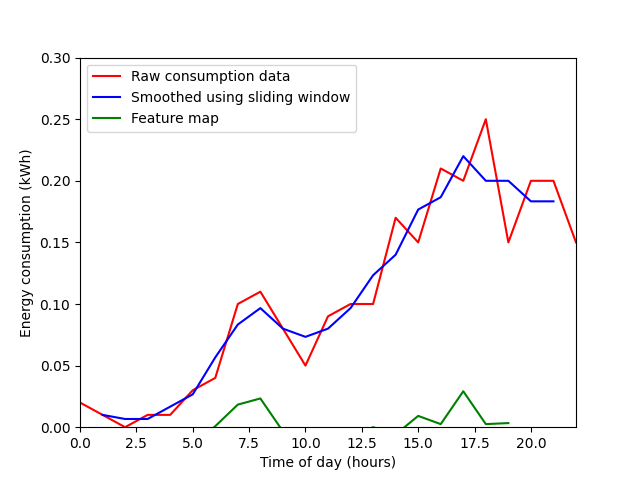
\includegraphics[scale=0.5]{img/prerequisites/energyConsumptionPlots.png}
    \caption{Effect of using a sliding window of size 3 with the averaging function to reduce noise in time series data, and feature map found by applying the kernel $\begin{bmatrix}-0.125 & -0.125 & 0.5 & -0.125 & -0.125 \end{bmatrix}$ to the smoothed data. For the feature map, the $y$-axis represents how well the given window matches the pattern defined by the kernel.}
    \label{fig:slidingWindowIllustration}
\end{figure}

Aplying a sliding window with an averaging function is a useful preprocessing step, but sliding windows can also be used to do actual analysis. A common operation to apply when using sliding windows for analysis is convolution.

\subsubsection{Convolutions for time series analysis}
In the context of vectors of finite length, the convolution operation is a method for assessing the presence of a pattern in a vector. Formally, the convolution operation is defined as follows\footnote{This is actually the cross-correlation operation, but in a machine learning context, the two operations are used interchangeably}:

\begin{equation}\label{eq:1dconvolution}
    [\boldsymbol{w} \circledast \boldsymbol{x}]i = \sum_u^{L-1} w_u x_{i+u}
\end{equation}

where $\boldsymbol{w}$ is a the weight vector, which defines the pattern to detect, $\boldsymbol{x}$ is the vector to be analysed, and $L$ is the length of $\boldsymbol{w}$. $\boldsymbol{w}$ is called the \emph{kernel}, and the output of the convolution is called the \emph{feature map}. One can then imagine sliding $\boldsymbol{w}$ across an input vector $\boldsymbol{x}$ which is longer than $\boldsymbol{w}$ to see where in $\boldsymbol{x}$ the pattern defined by $\boldsymbol{w}$ is present. An illustration of this is shown in figure \ref{fig:slidingWindowIllustration}. Here, the kernel $\begin{bmatrix}-0.125 & -0.125 & 0.5 & -0.125 & -0.125 \end{bmatrix}$ is applied to the smoothed energy consumption data. Intuitively, this kernel finds instances of peaks; it rewards high values in the center of the window, and penalises high values in the edges. Using this kernel, we were able to identify two peaks; one in the morning and one in the afternoon. Of course, convolution can be used to identify much more complex patterns than peaks. Ideally, one would have a machine learning model learn which patterns are the most useful, and learn the kernels which capture them.

Equation \ref{eq:1dconvolution} shows how to apply the convolution operation to a one-dimensional vector. This is useful when analysing univariate time series, but for multivariate time series we may want to find patterns between variables. In this case, we can define a two dimensional kernel $\mathbf{W}$, and define the convolution operation as follows:

\begin{equation}\label{eq:2dconvolution}
    [\mathbf{W} \circledast \mathbf{X}]_{i,j} = \sum_u^W \sum_v^H w_{u,v}x_{i+u,j+v}
\end{equation}
where $\mathbf{W}\in \mathbb{R}^{W\times H}$.

%pros, cons

\subsubsection{Shapelets}
%pros, cons
